Distributed systems typically consist of two or more components that communicate \emph{asynchronously} by sending and receiving messages through a network layer. When a component receives a message, it responds by executing a predefined \emph{message handler}. This handler consists of a sequence of program statements that might update the internal state of the component, send a message to another component in the system, or even create an entirely new component.

As an example of a distributed system, Figure~\ref{fig:azurestore} shows the top-level components of Azure Storage vNext, a distributed extent management system for Windows Azure that is used in production inside Microsoft. Azure Storage vNext consists of multiple extent managers, extent nodes and a remote procedure call (RPC) communication engine. Each extent manager is responsible for managing a subset of the extent nodes. Each extent node is responsible for storing its corresponding extent in a local storage. Finally, the RPC engine is responsible for sending messages across the network, and enqueuing any received messages in the inbox queue of the corresponding node. This system is described in more details in Section~\ref{sec:cases:azurestore}.

\subsection{Finding bugs in distributed systems}
\label{sec:overview:bugs}

Due to the asynchronous nature of message passing, message handlers can potentially interleave in arbitrary order. To complicate matters further, random failures are the norm in distributed systems that operate in production: nodes might fail at any moment in a cluster, and thus programmers have to implement sophisticated mechanisms that can deal with these failures and appropriately recover the state of the system. Also, with multicore machines becoming a commodity nowadays, individual components of a distributed system are commonly implemented using multithreaded code, which adds another source of nondeterminism.

To be able to efficiently find bugs in a distributed system and deterministically reproduce them, a testing tool must provide three key capabilities: capturing all sources of nondeterminism; injecting faults in arbitrary interleavings; and exploring all possible interleavings in a systematic fashion. Traditional testing techniques used by product groups, although focus on stressing the system and randomly injecting faults, they are typically unable to capture and control all sources of nondeterminism, which makes them ineffective in finding the most tricky of bugs.

\begin{figure}[t]
\centering
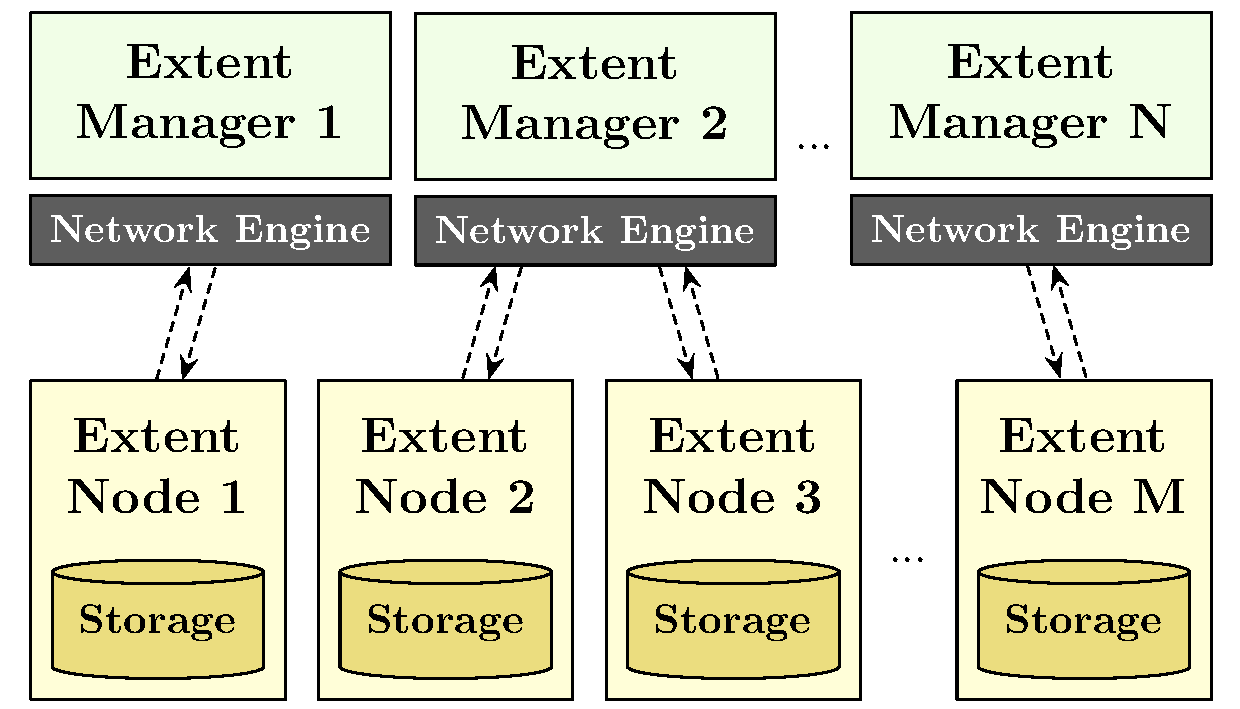
\includegraphics[width=\linewidth]{img/azurestore}
\caption{High-level architecture of a distributed extent management system for Windows Azure.}
\label{fig:azurestore}
\end{figure}

How cheng was testing his code before and how after -- high level, pretty picture

